\documentclass[dvipdfmx,tikz]{standalone}
\usepackage{tikz}
\usepackage{ifthen}


\usetikzlibrary{
  shapes,
  shapes.geometric,
  arrows.meta,
  calc,
}

\definecolor{cA}{HTML}{0072BD}
\definecolor{cB}{HTML}{EDB120}
\definecolor{cC}{HTML}{77AC30}
\definecolor{cD}{HTML}{D95319}

\begin{document}
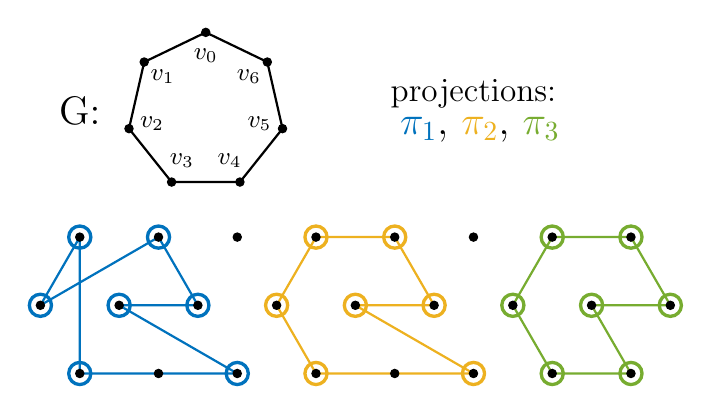
\begin{tikzpicture}
  \foreach \x in {0,...,2}{
      \pgfmathsetmacro{\range}{ifthenelse(mod(\x,2)==1,8,7)}
      \foreach \y in {0,...,\range}{
          \pgfmathsetmacro\shift{mod(\x,2)*0.5}
          \coordinate (a\x\y) at ({\y - \shift},{-sqrt(3)/2*\x});
        }}

  \foreach \xy in {00,10,01,12,11,22,20}{
      \draw[cA,very thick] (a\xy) circle (4pt);
    }
  \draw[cA,thick] (a00) -- (a10) -- (a01) -- (a12) -- (a11) -- (a22) -- (a20) -- (a00);

  \foreach \xy in {13,03,04,15,14,25,23}{
      \draw[cB,very thick] (a\xy) circle (4pt);
    }
  \draw[cB,thick] (a13) -- (a03) -- (a04) -- (a15) -- (a14) -- (a25) -- (a23) -- (a13);

  \foreach \xy in {16,06,07,18,17,27,26}{
      \draw[cC,very thick] (a\xy) circle (4pt);
    }
  \draw[cC,thick] (a16) -- (a06) -- (a07) -- (a18) -- (a17) -- (a27) -- (a26) -- (a16);

  \foreach \x in {0,...,2}{
      \pgfmathsetmacro{\range}{ifthenelse(mod(\x,2)==1,8,7)}
      \foreach \y in {0,...,\range}{
          \filldraw[draw=black,fill=black] (a\x\y) circle (1.5pt);
        }
    }

  \begin{scope}[xshift=1.6cm,yshift=1.6cm]
    \foreach \i in {0,...,6}{
        \pgfmathsetmacro{\angle}{90+360/7*\i}
        \filldraw[draw=black,fill=black] (\angle:1) circle (1.5pt);
        \node at (\angle:0.7) {\small $v_\i$};
      }
    \node[regular polygon, regular polygon sides=7, minimum size=2cm, draw, thick] at (0,0) {};
  \end{scope}

  \node[anchor=center] at (0,1.6) {\Large G:};
  \node[anchor=center,align=center] at ($(a05)+(0,1.6)$) {
    \large{projections:}\\
    \Large{
      \textcolor{cA}{$\pi_1$}, \textcolor{cB}{$\pi_2$}, \textcolor{cC}{$\pi_3$}
    }};
\end{tikzpicture}
\end{document}
